

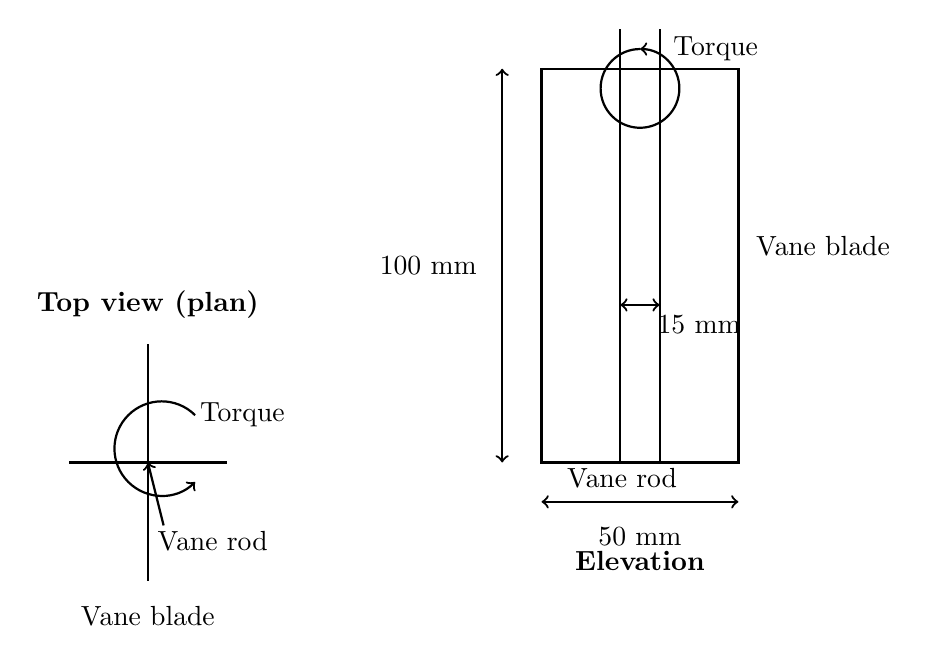
\begin{tikzpicture}

% Top View (Plan)
\begin{scope}[xshift=-5cm]
    % Vane rod (vertical line)
    \draw[thick] (0,0) -- (0,1.5);
    \draw[thick] (0,0) -- (0,-1.5);
    
    % Vane blade (horizontal line)
    \draw[thick] (-1,0) -- (1,0);

    % Torque arrow
    \draw[->, thick] (0.6,0.6) arc[start angle=45, end angle=315, radius=0.6];
    \node at (1.2,0.6) {Torque};

    % Labels
    \node[above] at (0,1.7) {\textbf{Top view (plan)}};
    \node[right] at (0,-1) {Vane rod};
    \node[below] at (0,-1.7) {Vane blade};
    \draw[->, thick] (0.2,-0.8) -- (0,0);
\end{scope}

% Elevation View (Side view)
% Rectangle for vane blade
\draw[thick] (0,0) rectangle (2.5,5);

% Vane rod (vertical lines in elevation view)
\draw[thick] (1.5,5.5) -- (1.5,0);
\draw[thick] (1,5.5) -- (1,0);

% Torque arrow in elevation view
\draw[->, thick] (1.25,5.25) arc[start angle=90, end angle=450, radius=0.5];
\node[right] at (1.55,5.25) {Torque};

% Dimensions
\draw[<->, thick] (-0.5,0) -- (-0.5,5);
\node[left] at (-0.7,2.5) {100 mm};

\draw[<->, thick] (0,-0.5) -- (2.5,-0.5);
\node[below] at (1.25,-0.7) {50 mm};

\draw[<->, thick] (1,2) -- (1.5,2);
\node[right] at (1.35,1.75) {15 mm};

% Labels
\node[below] at (1.25,-1) {\textbf{Elevation}};
\node[above right] at (2.6,2.5) {Vane blade};
\node[right] at (0.2,-0.2) {Vane rod};

\end{tikzpicture}


